\documentclass{beamer}
\usetheme{AnnArbor}
\usecolortheme{crane}

\title%[Crisis] % (optional, only for long titles)
{Dispositivo per pesatura arnie}
\subtitle{Configurazione con celle di carico}

\begin{document}

\frame{\titlepage}

%\begin{frame}
%\frametitle{Table of Contents}
%\tableofcontents[currentsection]
%\end{frame}


\section{Prime prove}
\begin{frame}
  \frametitle{Circuito e celle di carico}
  \begin{columns}[c] % the "c" option specifies center vertical alignment
    \column{.5\textwidth} % column designated by a command
      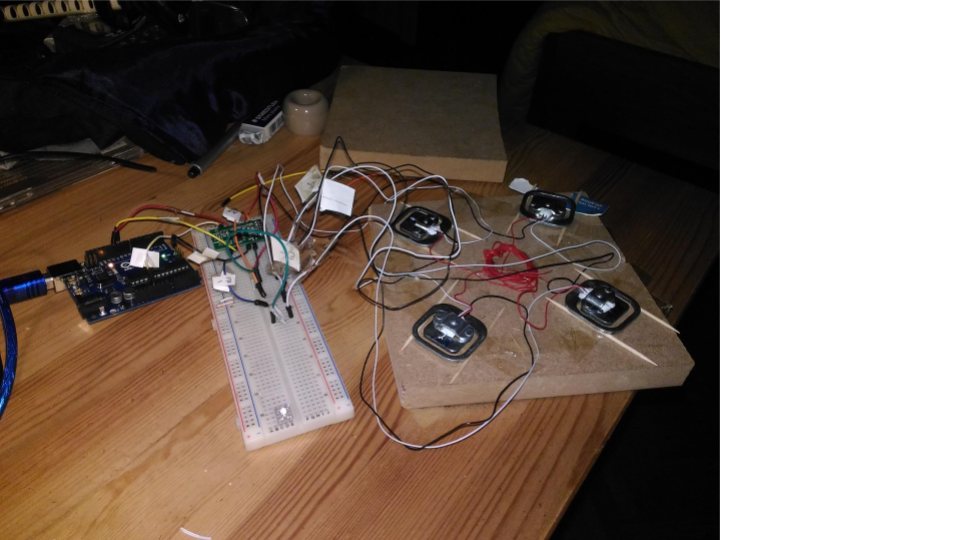
\includegraphics[height=4.5cm]{../Foto/Prime_prove/circuito.png}
    \column{.5\textwidth}
      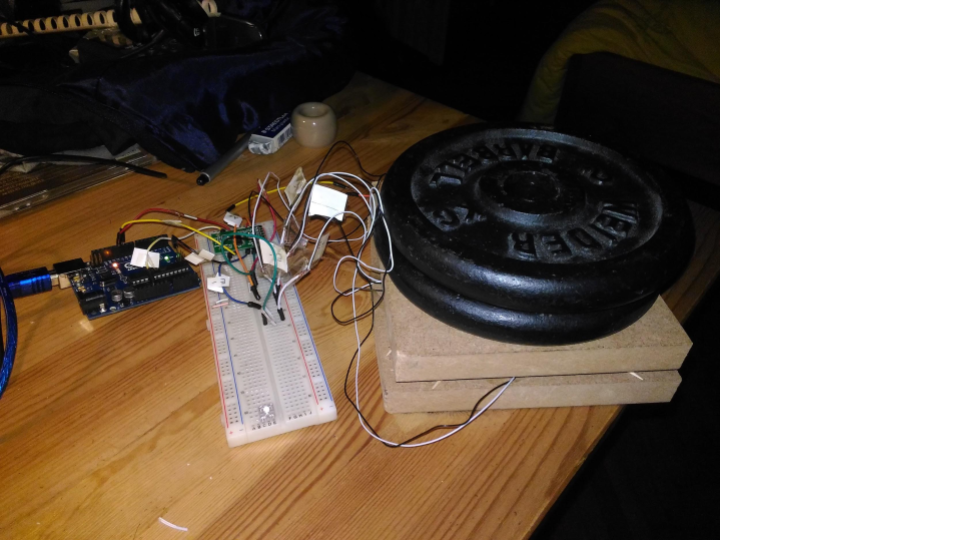
\includegraphics[height=4.5cm]{../Foto/Prime_prove/circuito_in_funzione.png}
  \end{columns}
\end{frame}
\begin{frame}
  \frametitle{Primi risultati}
  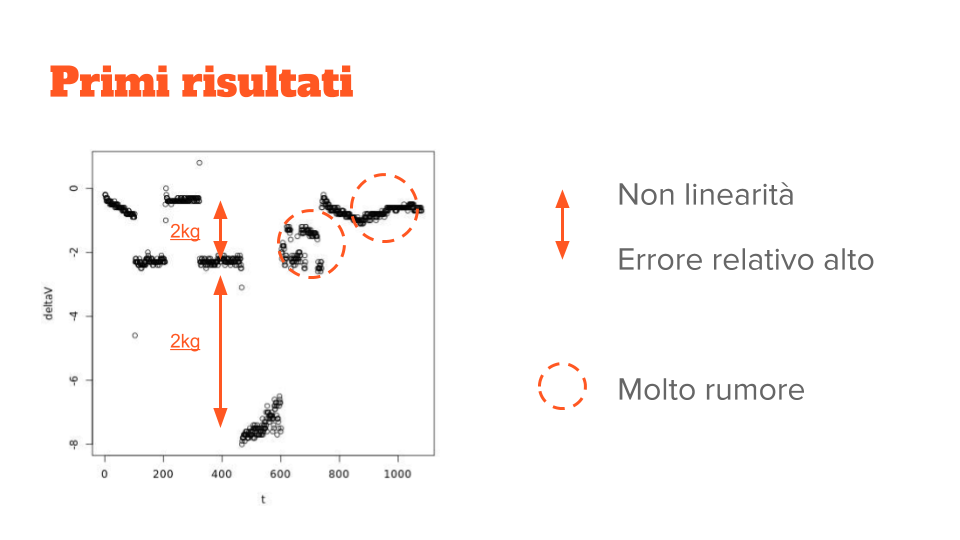
\includegraphics[width=11cm]{../Foto/Prime_prove/primi_risultati}
\end{frame}

\section{Saldatura e stabilit\`a}
\begin{frame}
  \frametitle{Saldatura}
  \begin{columns}[c] 
    \column{.5\textwidth} 
      \begin{itemize}
        \item la stabilit\`a migliora
        \item restano oscillazioni durante una giornata
      \end{itemize}
    \column{.5\textwidth}
      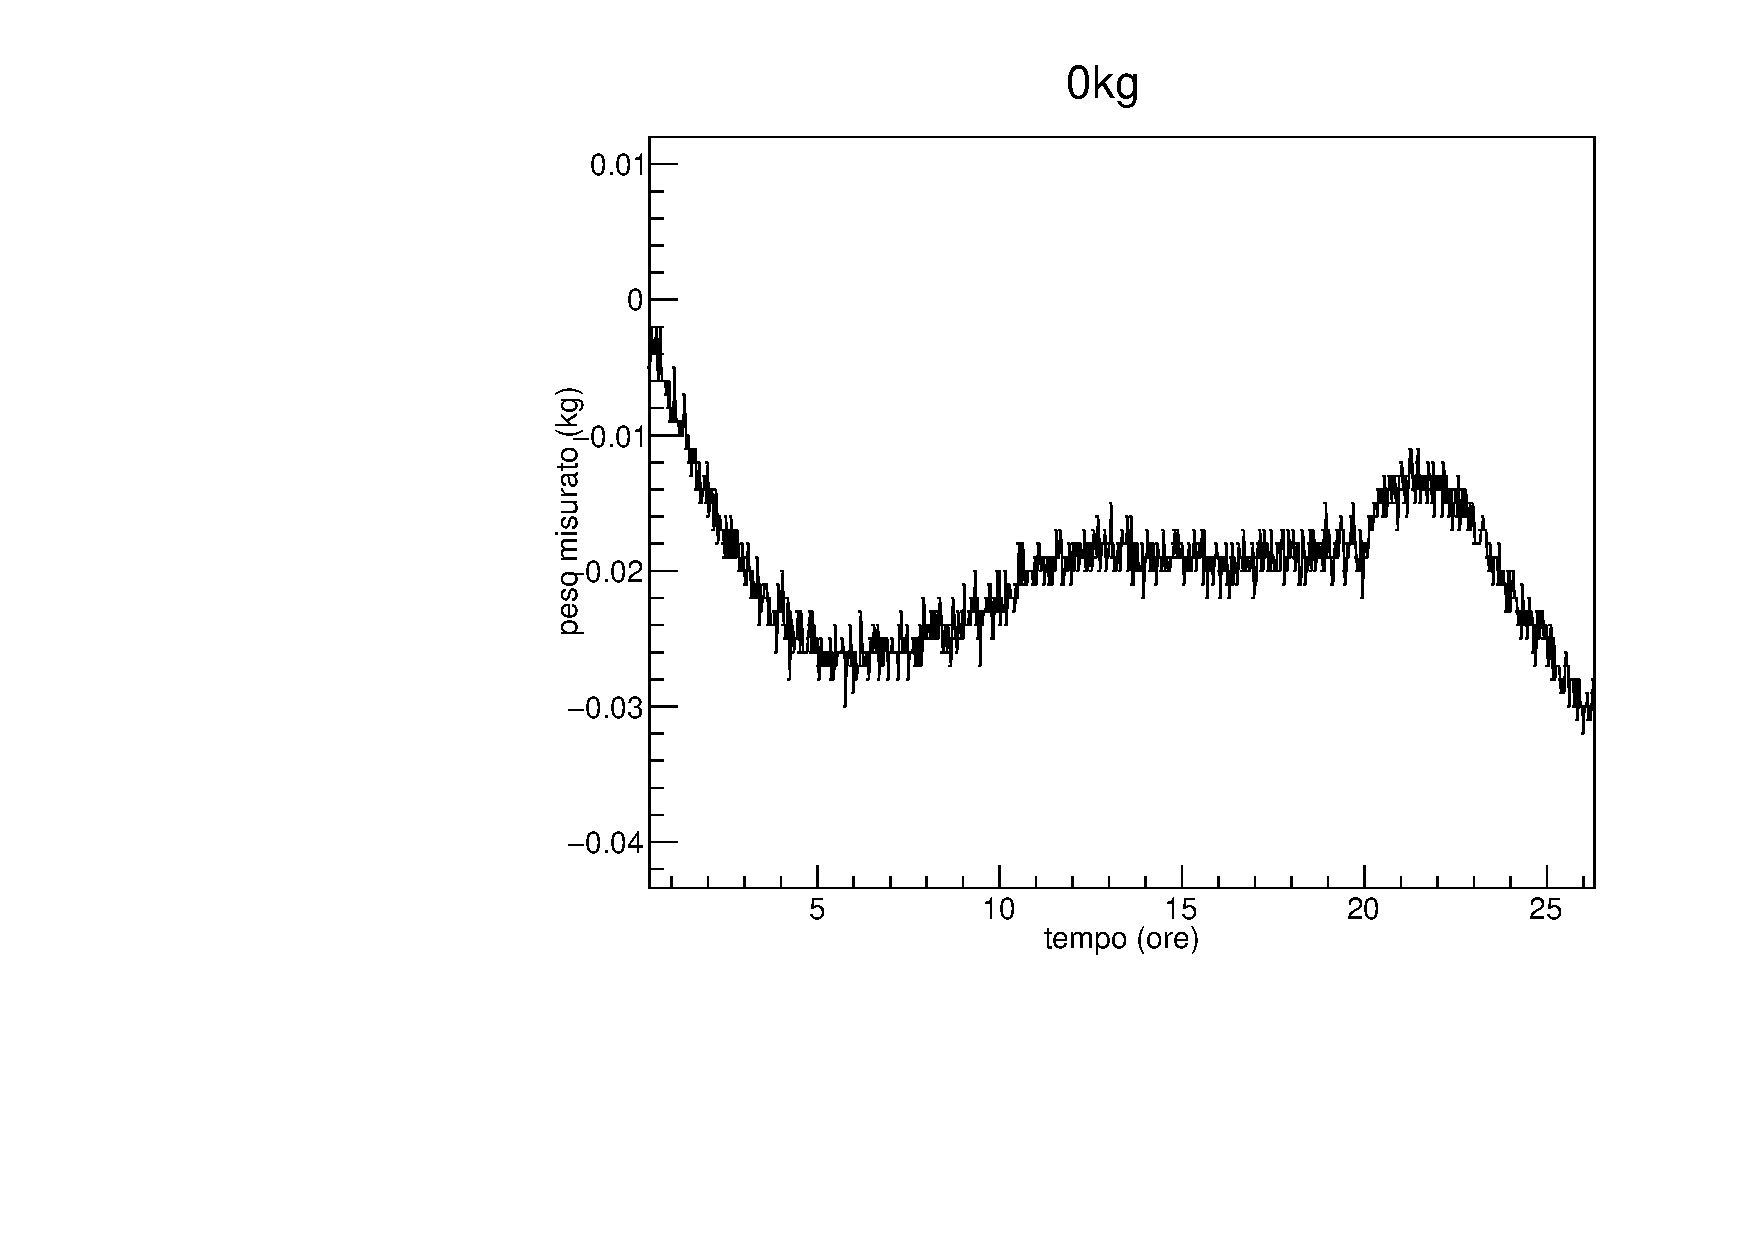
\includegraphics[height=5cm]{../../analisi_dati/background/0kg_24h}   
   \end{columns}
\end{frame}
\begin{frame}{Comportamento parabolico}
  \begin{columns}[c] 
    \column{.5\textwidth} 
      \begin{itemize}
        \item un fit conferma l'intuizione (buon chi2)
        \item possibile criterio per pulire i dati
      \end{itemize}
    \column{.5\textwidth}
      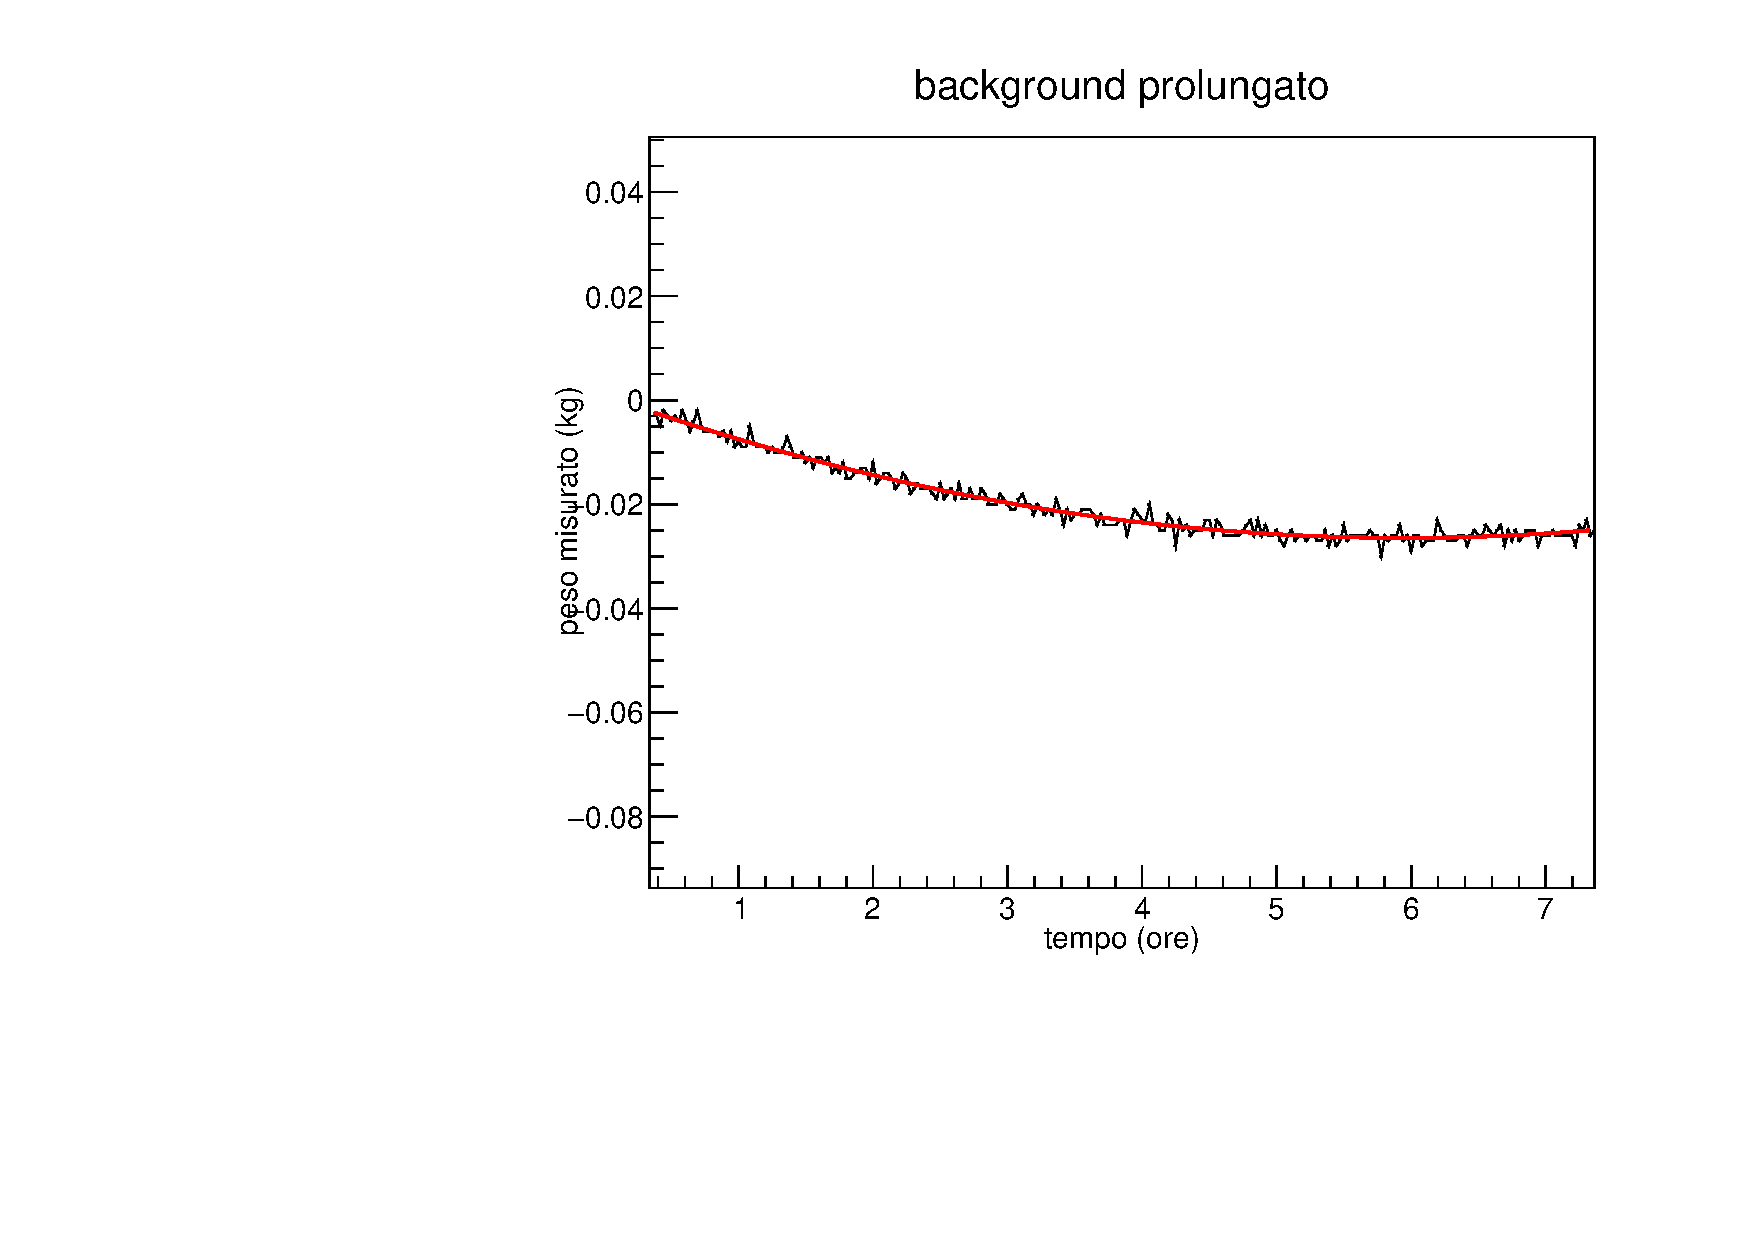
\includegraphics[height=5cm]{../../analisi_dati/background/0kg_parabola}   
   \end{columns}
\end{frame}
\begin{frame}{Stabilit\`a}
  \begin{columns}[c]
    \column{.5\textwidth}
      \large{60 ore, peso variato}
      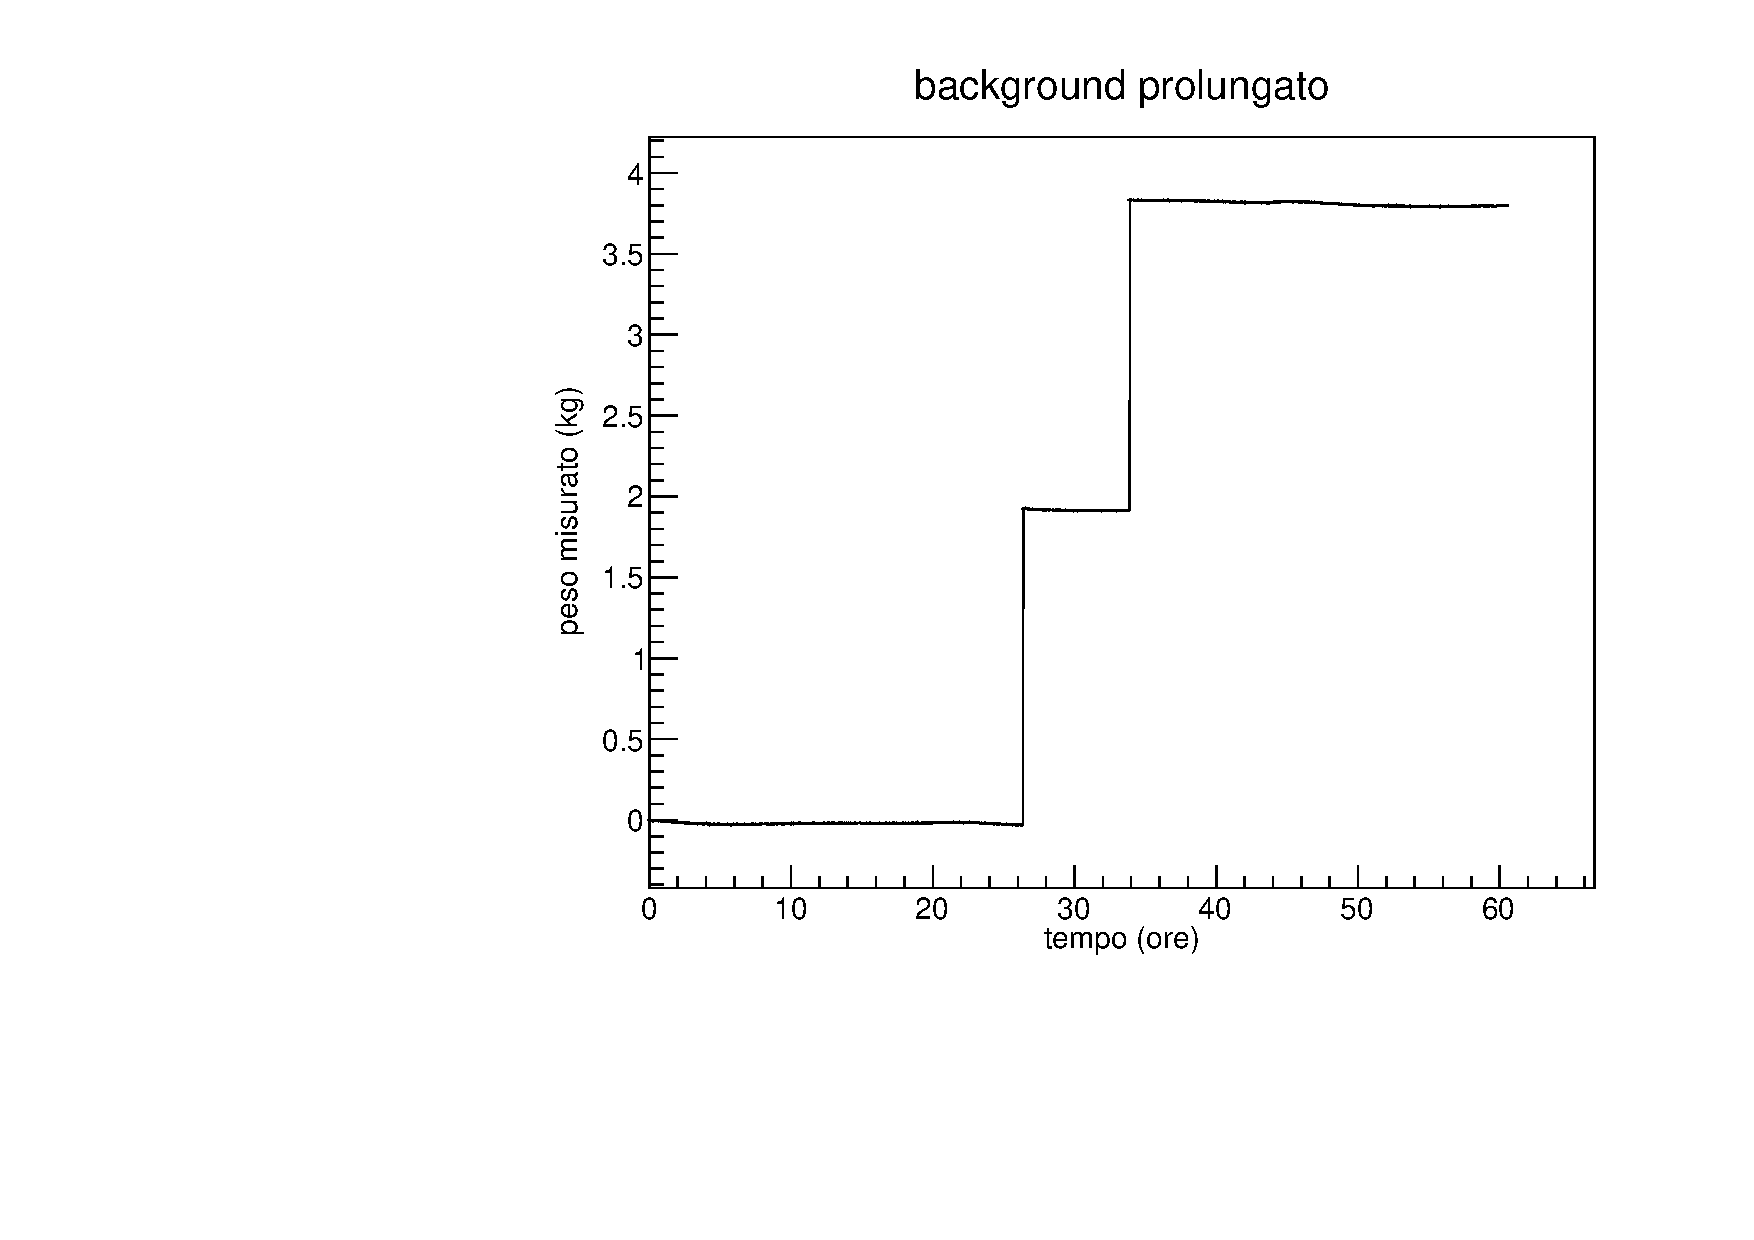
\includegraphics[height=5cm]{../../analisi_dati/background/60h}
    \column{.5\textwidth}
      \large{8 giorni, peso fissato}
      \\\small{(scarto di 120g)}
      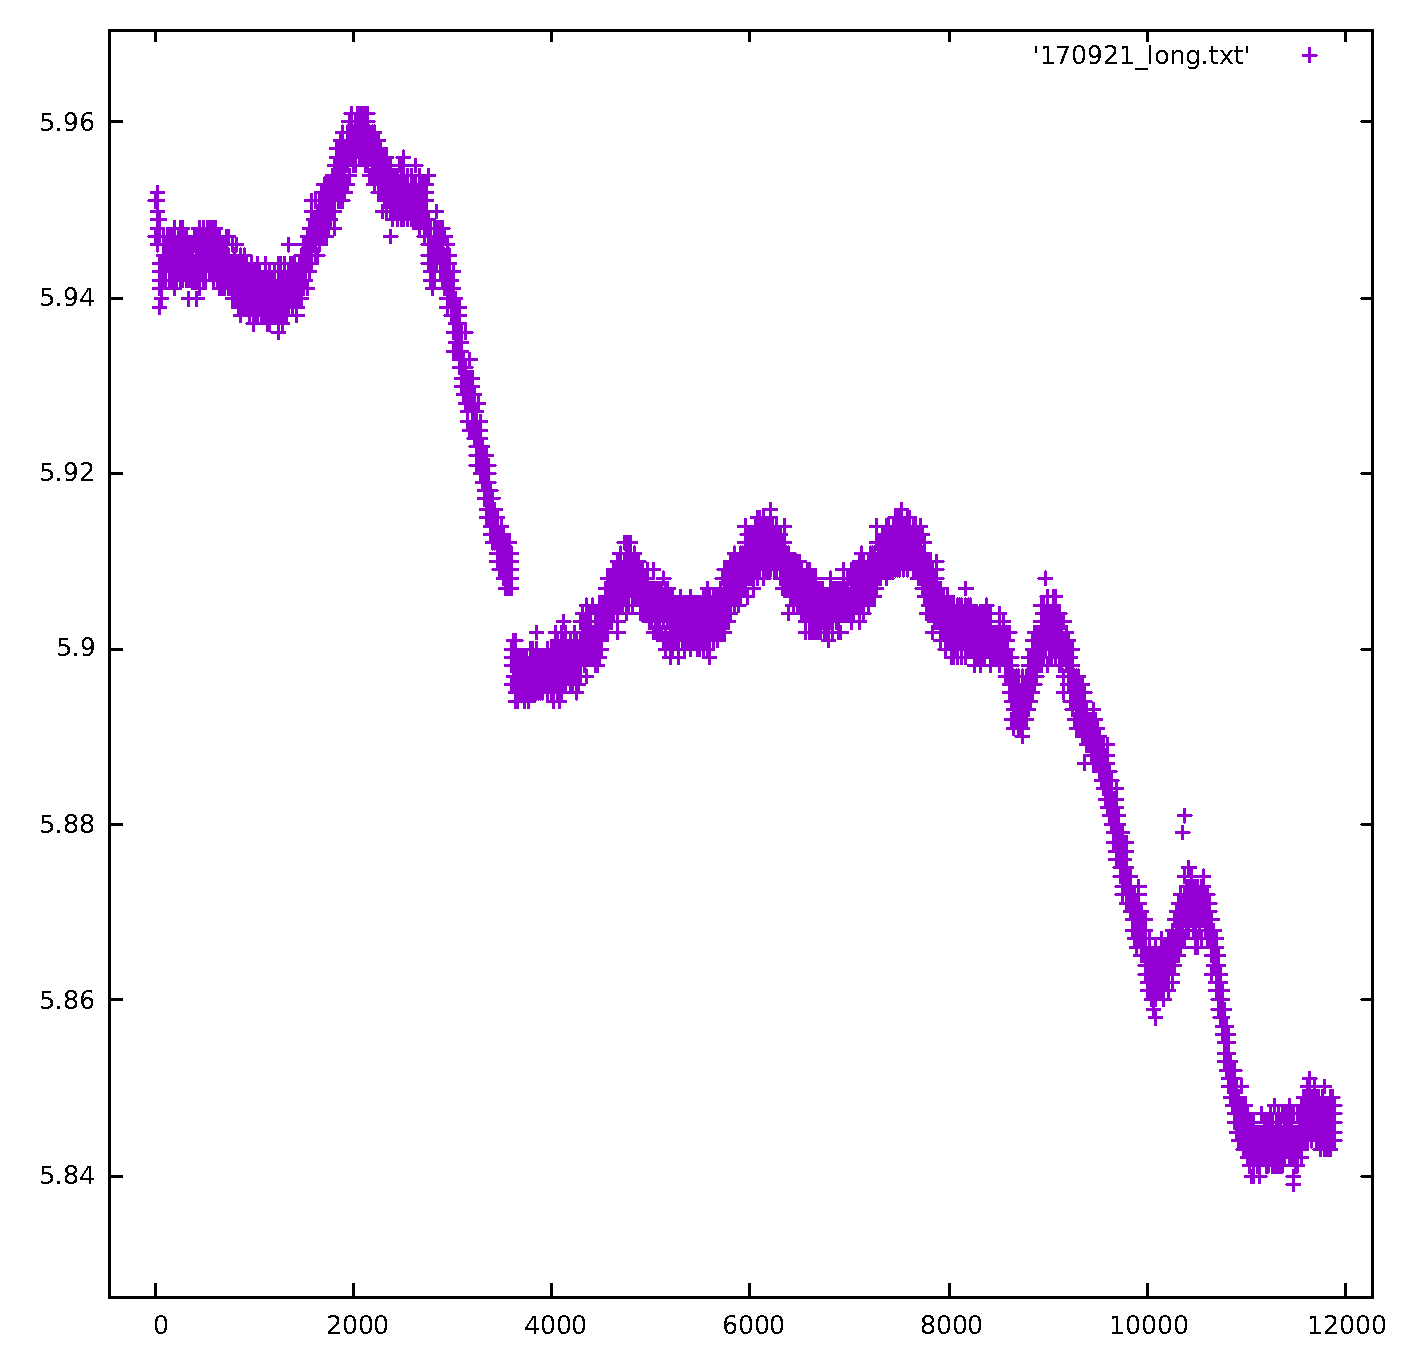
\includegraphics[height=5cm]{../../analisi_dati/background/8gg}
    \end{columns}
\end{frame}

\section{Misure di temperatura}
\begin{frame}{Sensore DHT11}
  \begin{columns}[c] 
    \column{.1\textwidth}
    \column{.5\textwidth} 
      misure di 
      \begin{itemize}
        \item temperatura
        \item umidit\`a
      \end{itemize}
    \column{.4\textwidth}
      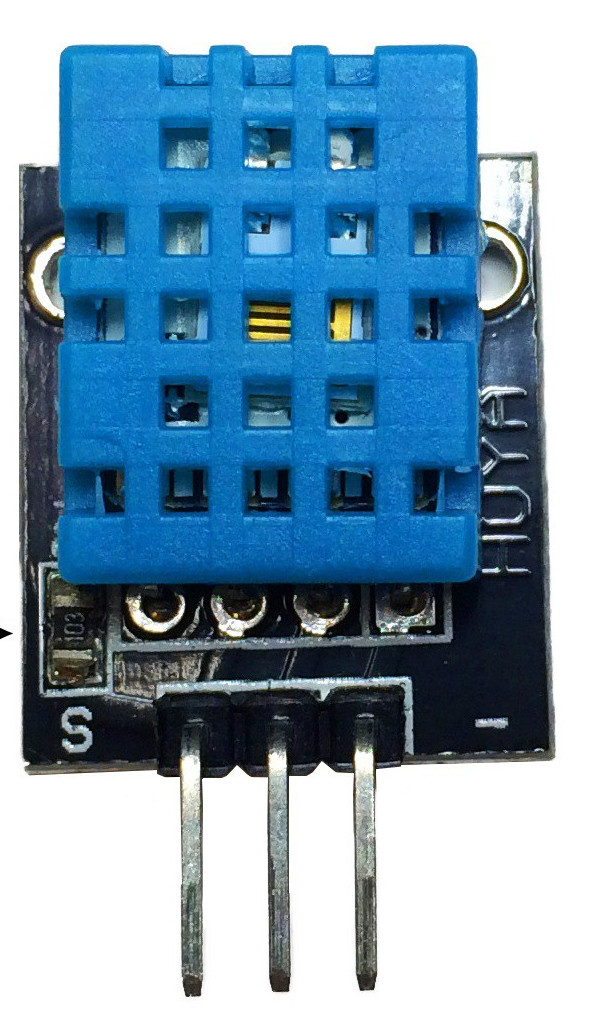
\includegraphics[height=5cm]{../Foto/DHT11}
   \end{columns}
\end{frame}
\begin{frame}{Risultati complessivi}
  correlazioni tra temperatura e peso? (periodicit\`a)
  \begin{columns}[c] 
    \column{.5\textwidth} 
      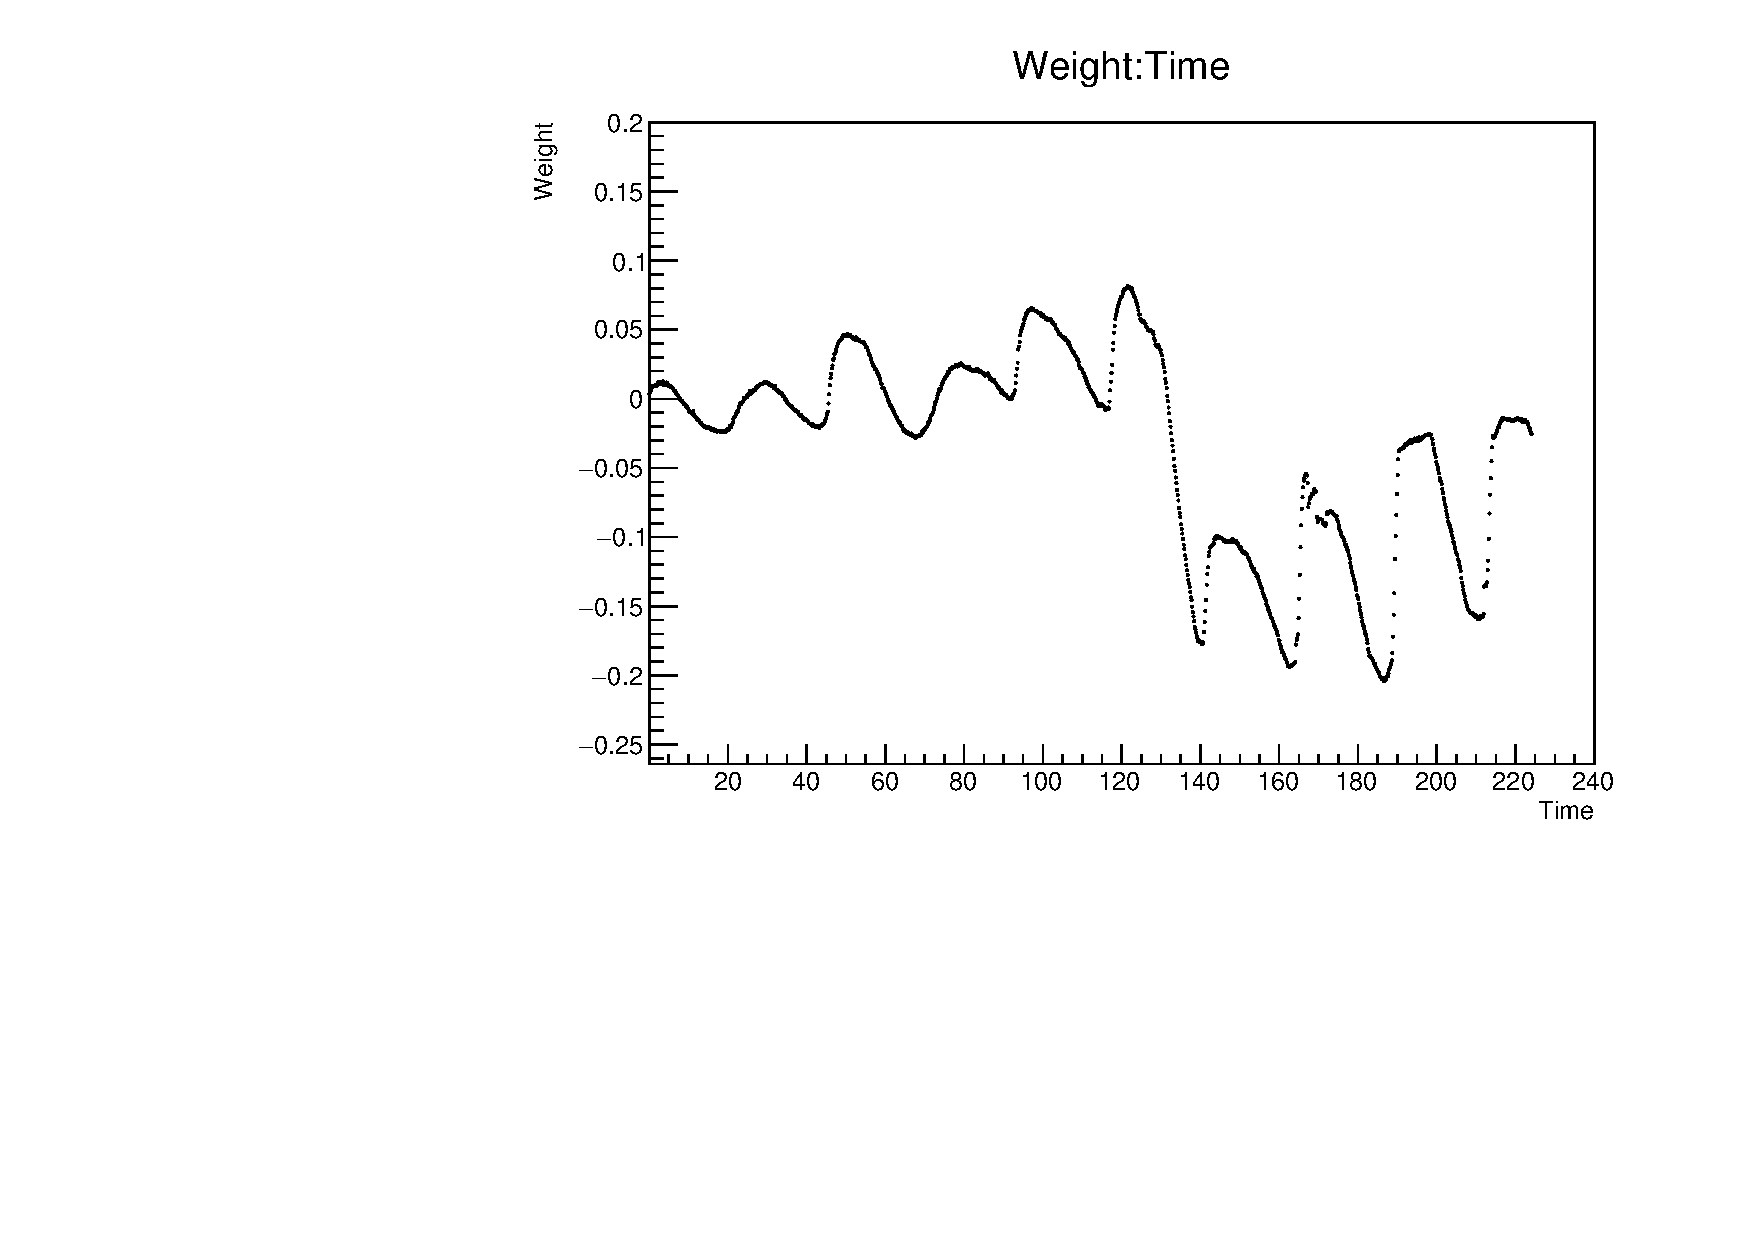
\includegraphics[height=4.5cm]{../../analisi_dati/171010_long_sd_temp/M_Weight}
    \column{.5\textwidth}
      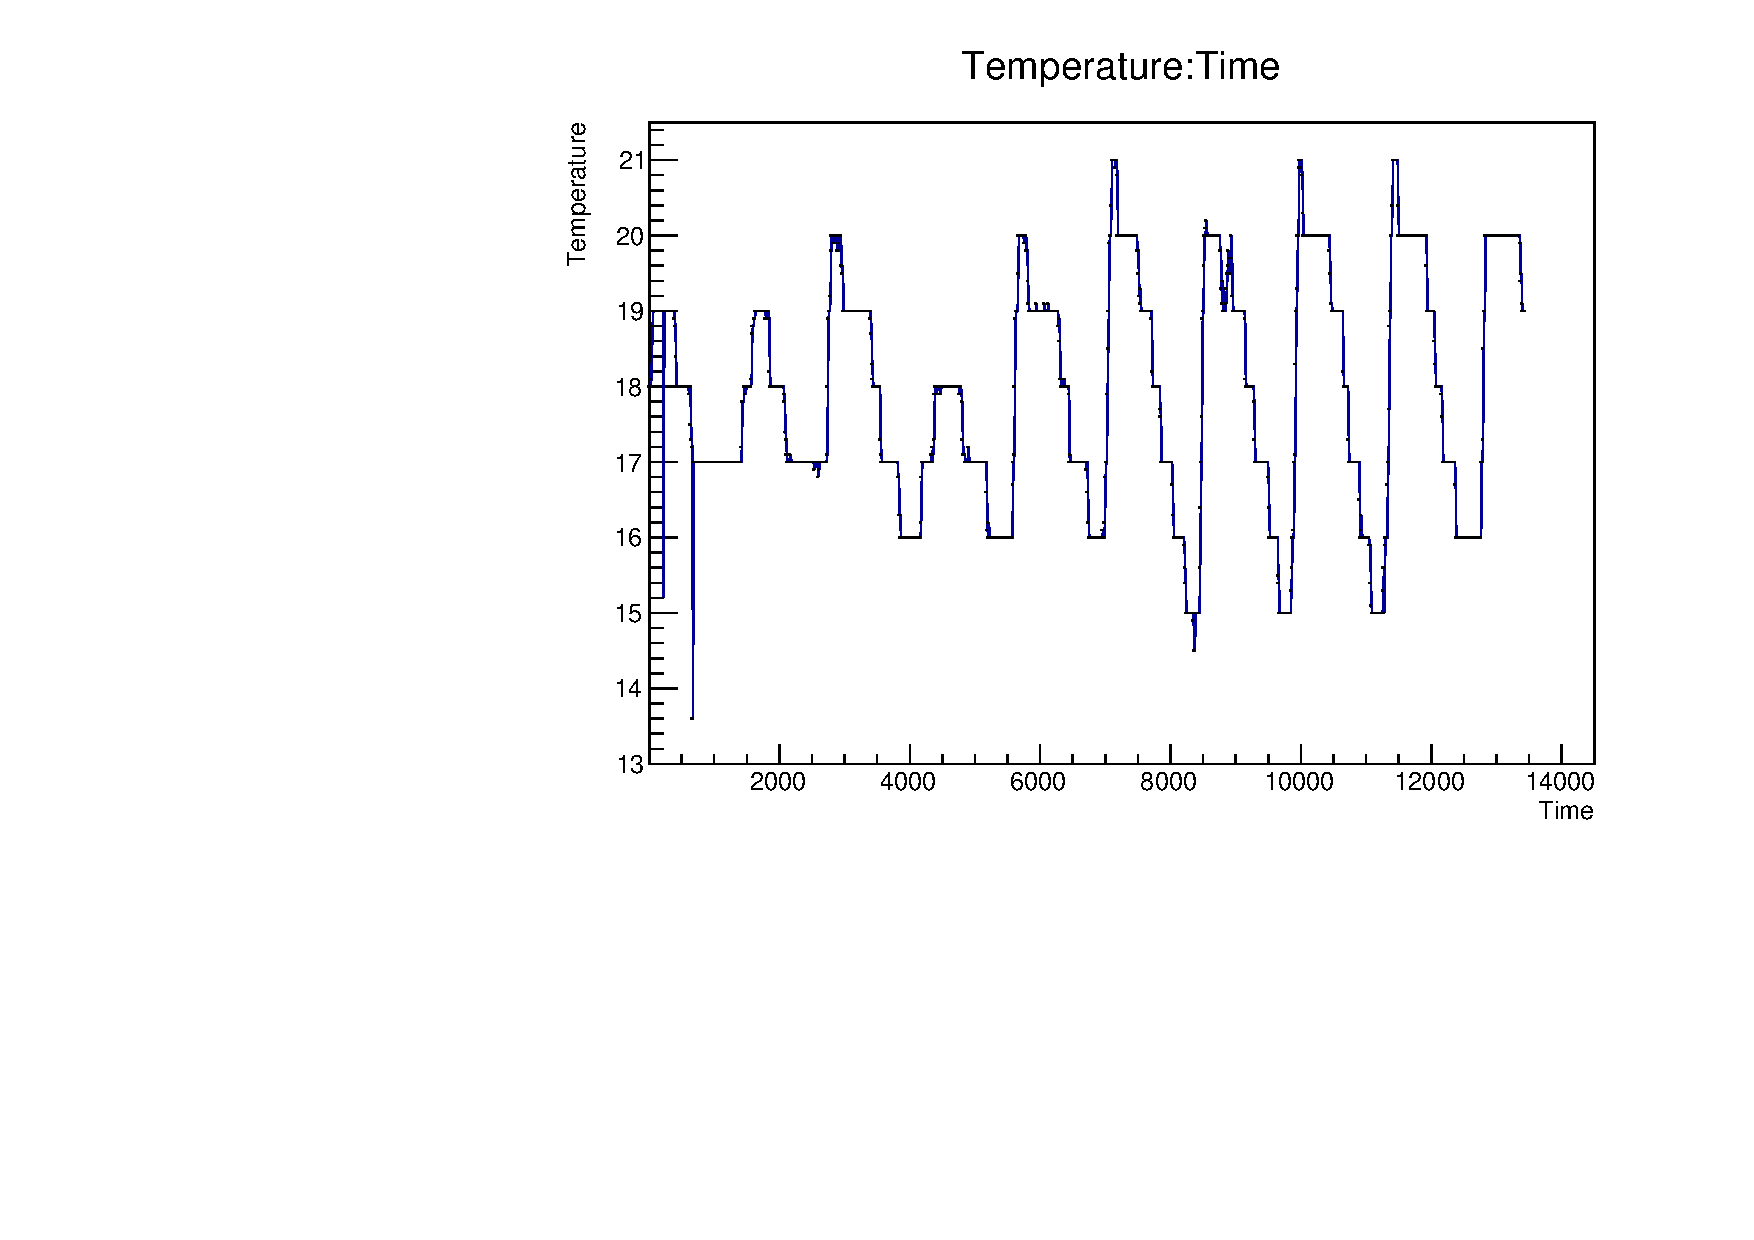
\includegraphics[height=4.5cm]{../../analisi_dati/171010_long_sd_temp/M_Temperature}   
   \end{columns}
\end{frame}
\begin{frame}{Correlazione temperatura-peso}
  prima/dopo la caduta
  \begin{columns}[c] 
    \column{.5\textwidth} 
      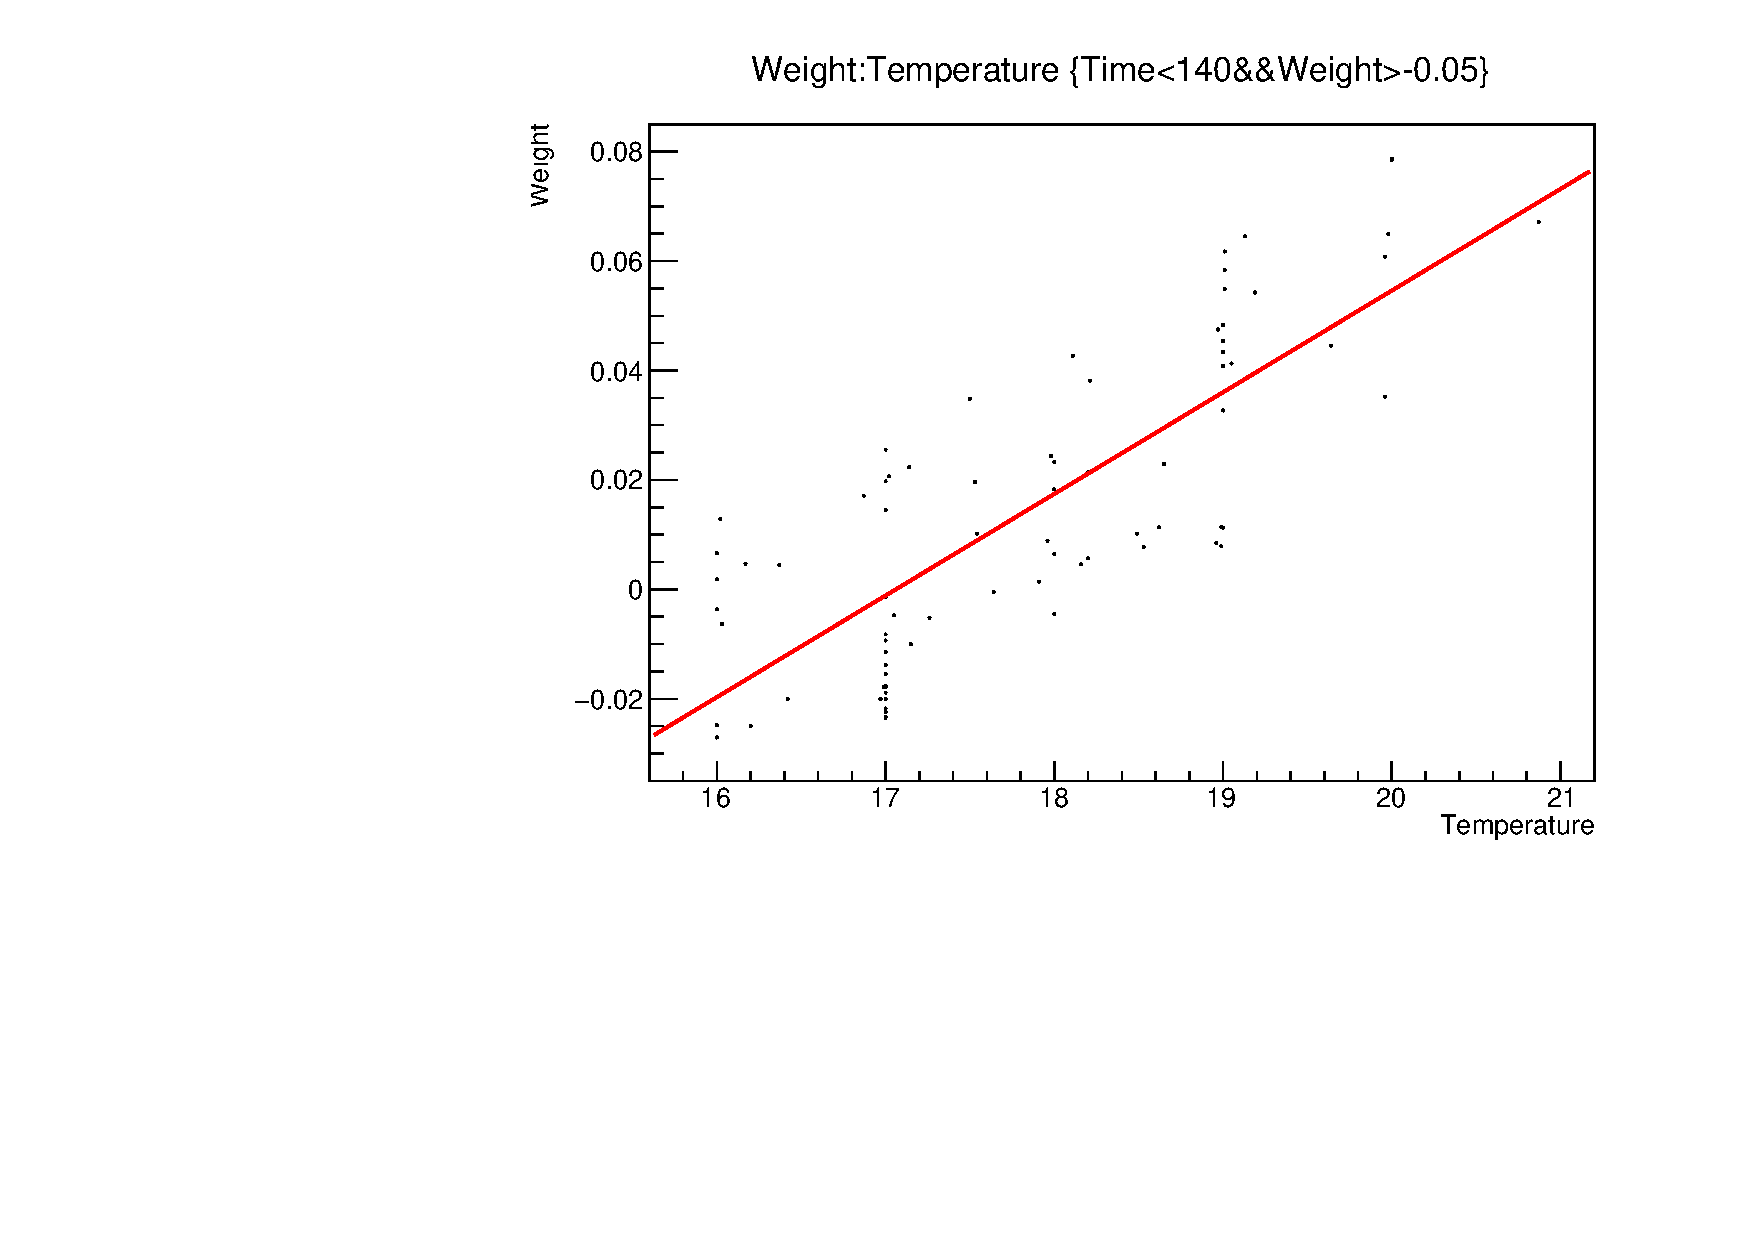
\includegraphics[height=4.5cm]{../../analisi_dati/171010_long_sd_temp/Weight:Temperature_timed_first}
    \column{.5\textwidth}
      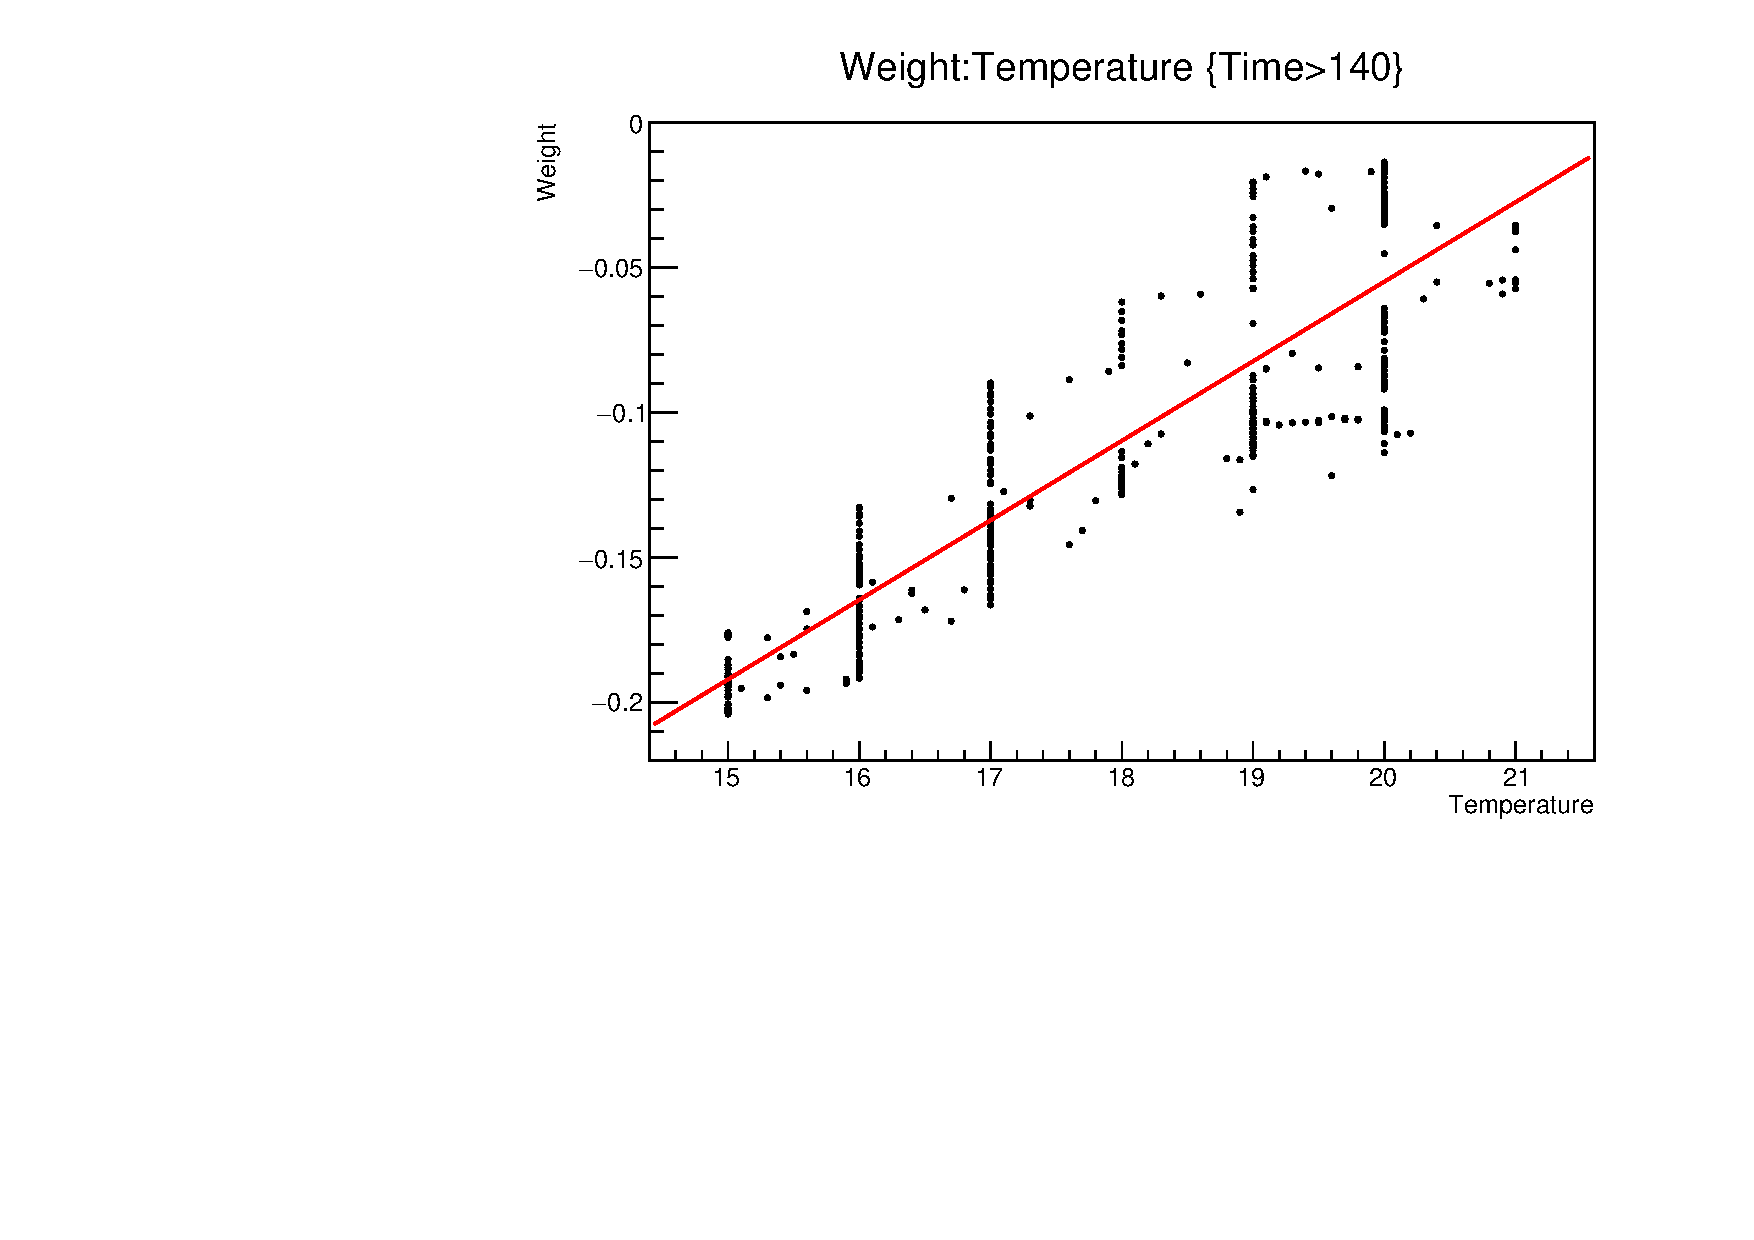
\includegraphics[height=4.5cm]{../../analisi_dati/171010_long_sd_temp/Weight:Temperature_timed_second}
   \end{columns}
\end{frame}

\section{Harware senza fili}
\begin{frame}
  \Large{Prossimi step}
  \begin{itemize}
    \item nuovo hardware (NodeMCU) con connessione Wi-Fi
    \item analisi dati su periodi pi\`u lunghi
    \item raccolta dati con peso variabile (ordine della produzione delle api)
  \end{itemize}
\end{frame}


\end{document}
